
\documentclass{beamer}
\usepackage[latin1]{inputenc}
%\usetheme{Montpellier}
%\usetheme{Boadilla}
%\usecolortheme[RGB={204,51,255}]{structure}
%\usecolortheme[named=purple]{structure}
%\usecolortheme[RGB={62,128,62}]{structure}
\usecolortheme[RGB={62,62,128}]{structure}
%\definecolor{reddish}{rgb}{0.3,0.15,0.3}
%\definecolor{light}{rgb}{0.8,0.6,0.8}
%\definecolor{reddish}{rgb}{.5,0.15,0.15}
\definecolor{reddish}{rgb}{0.5,0.3,0.4}
%\definecolor{light}{rgb}{0.8,0.6,0.8}
\definecolor{reddish}{rgb}{.7,0.25,0.25}
\definecolor{greenish}{rgb}{.25,0.8,0.25}
\definecolor{blueish}{rgb}{.25,0.25,0.7}
\definecolor{purple}{rgb}{.5,0.0,0.5}
\usepackage{graphicx}
\usepackage{pstricks}
\usepackage{epsfig}
\newcommand{\btVFill}{\vskip0pt plus 1filll}

\setbeamertemplate{navigation symbols}{}

\newcommand{\crish}{\color{reddish}}
\newcommand{\cgish}{\color{greenish}}
\newcommand{\cbla}{\color{black}}
\newcommand{\cred}{\color{red}}
\newcommand{\cblu}{\color{blue}}
\newcommand{\cgrish}{\color{green}}

\newcommand{\sm}{\color{reddish}$}
\newcommand{\fm}{$\color{black}{}}

\newcommand{\letter}[1]{\color{blue}\texttt{#1}\color{black}}
 \newcommand{\binary}[1]{\color{red}\texttt{#1}\color{black}}

\usepackage{tikz}
\usetikzlibrary{arrows,decorations.markings,positioning}
\usepackage{epstopdf}
\usetikzlibrary{fit}
\usepackage{pgfplots}

\title[The Bayesian Brain lecture 3]{The Kalman filter: the Bayesian Brain lecture 3}
\author{COMSM0075 Information Processing and Brain}
\institute{\texttt{comsm0075.github.io}}
\date{October 2020}

\begin{document}

\maketitle


\pgfmathdeclarefunction{gauss}{2}{%
  \pgfmathparse{1/(#2*sqrt(2*pi))*exp(-((x-#1)^2)/(2*#2^2))}%
}

\begin{frame}{Kalman filter}
  \begin{quote}
The Kalman filter uses Bayesian fusion to estimate location based on noisy measurement and on dead reckoning.
  \end{quote}

\end{frame}

\begin{frame}{The problem}
\begin{center}
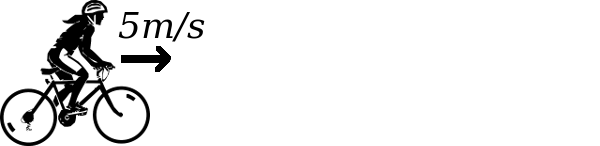
\includegraphics[width=6cm]{cyclist1.png}
\end{center}
\end{frame}


\begin{frame}{Dead reckoning}
\begin{center}
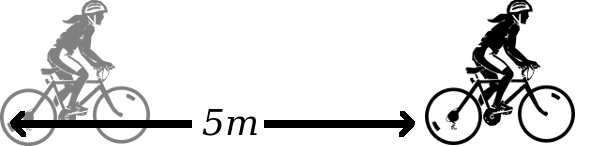
\includegraphics[width=6cm]{cyclist2.png}
\end{center}
\end{frame}


\begin{frame}{Measurement}
\begin{center}
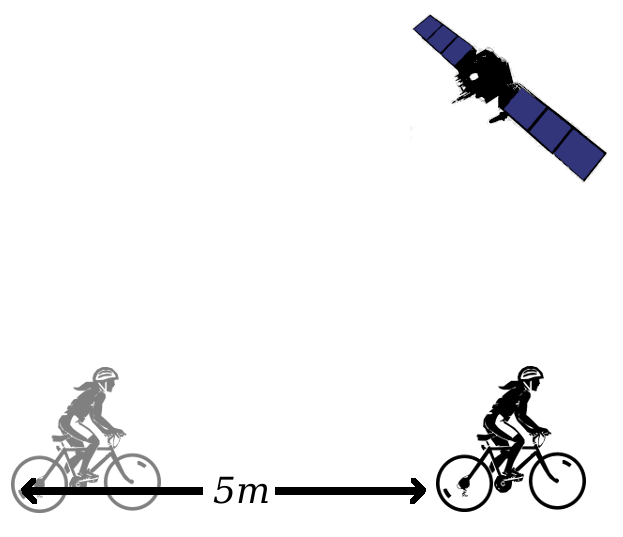
\includegraphics[width=6cm]{cyclist_gps.png}
\end{center}
\end{frame}


\begin{frame}{Two sources of position}
\begin{center}
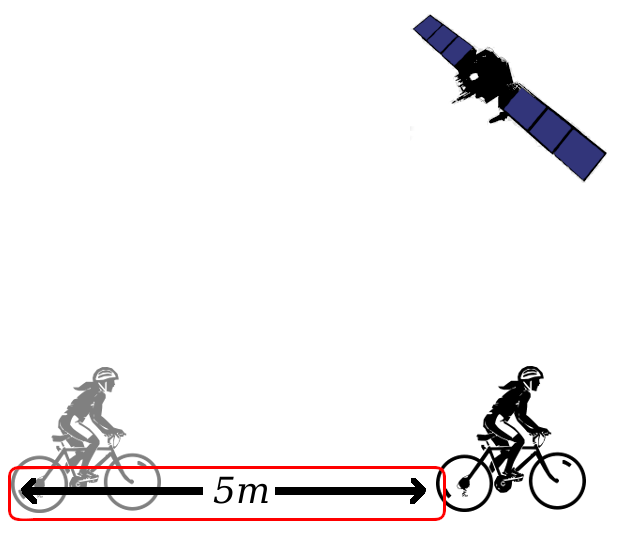
\includegraphics[width=6cm]{cyclist_gps1.png}
\end{center}
\end{frame}


\begin{frame}{Two sources of position}
\begin{center}
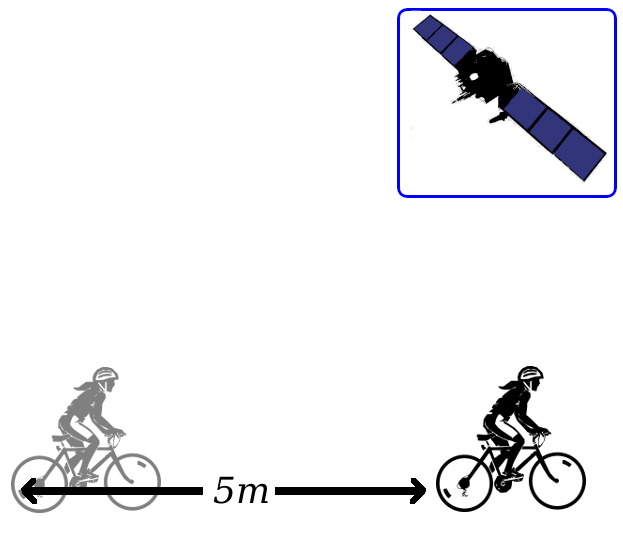
\includegraphics[width=6cm]{cyclist_gps2.png}
\end{center}
\end{frame}


\begin{frame}{Everything is Gau\ss{}ian}
1) specified by the mean and variance: \cblu$\mu=4$\cbla{} and \cblu$\sigma^2=1$\cbla{}
  \vskip 1cm
\begin{tikzpicture}
  \begin{axis}[
  no markers, domain=0:8, samples=100,
  axis lines*=left, xlabel=$x$, ylabel=$y$,
  every axis y label/.style={at=(current axis.above origin),anchor=south},
  every axis x label/.style={at=(current axis.right of origin),anchor=west},
  height=5cm, width=12cm,
  xtick={4}, ytick=\empty,
  xtick=\empty,
  ytick=\empty,
  enlargelimits=false, clip=false, axis on top,
  grid = major
  ]
  \addplot [very thick,blue] {gauss(4,1)};
\end{axis}
  \draw (8.25,2.2) node{\color{blue}$p(x)\sim \mathcal{N}(\mu,\sigma^2)$\cbla};
\end{tikzpicture}
\end{frame}


\begin{frame}{Everything is Gau\ss{}ian}
2) start with Gau\ss{}ians and stay with Gau\ss{}ians - Bayesian fusion
  \vskip 1cm
  \begin{tikzpicture}
  \begin{axis}[
  no markers, domain=0:8, samples=100,
  axis lines*=left, xlabel=$x$, ylabel=$y$,
  every axis y label/.style={at=(current axis.above origin),anchor=south},
  every axis x label/.style={at=(current axis.right of origin),anchor=west},
  height=5cm, width=12cm,
  xtick={4}, ytick=\empty,
  xtick=\empty,
  ytick=\empty,
  enlargelimits=false, clip=false, axis on top,
  grid = major
    ]
    \addplot [very thick,blue] {gauss(4,1)};
    \addplot [very thick,red] {gauss(2,2)};
    \addplot [very thick,black] {gauss(3.56,0.9)};
\end{axis}
\end{tikzpicture}
\end{frame}


\begin{frame}{Everything is Gau\ss{}ian}
2) start with Gau\ss{}ians and stay with Gau\ss{}ian - $Z\crish=\cblu{}X\crish+\cred{}Y$\cbla
  \vskip 1cm
  \begin{tikzpicture}
  \begin{axis}[
  no markers, domain=0:8, samples=100,
  axis lines*=left, xlabel=$x$, ylabel=$y$,
  every axis y label/.style={at=(current axis.above origin),anchor=south},
  every axis x label/.style={at=(current axis.right of origin),anchor=west},
  height=5cm, width=12cm,
  xtick={4}, ytick=\empty,
  xtick=\empty,
  ytick=\empty,
  enlargelimits=false, clip=false, axis on top,
  grid = major
    ]
    \addplot [very thick,blue] {gauss(3,1)};
    \addplot [very thick,red] {gauss(1,0.5)};
    \addplot [very thick,black] {gauss(4,1.12)};
\end{axis}
\end{tikzpicture}
\end{frame}



\begin{frame}{Some equations}
  \crish$$
  \mathbf{x}=\left(\begin{array}{c}s\\v\end{array}\right)
  $$\cbla{}
  {represents the position and
  speed, sometimes we have random variables:}
    \crish$$
  \mathbf{X}=\left(\begin{array}{c}S\\V\end{array}\right)
  $$\cbla{}
\end{frame}

\begin{frame}{Covariance}
\crish$$
P_{ij}=\langle (X_i-\bar{x}_i)(X_j-\bar{x}_j)\rangle
$$\cbla{}
{The idea is to update both the mean and the covariance; which is
equivalent for Gau\ss{}ian distributions to updating the distribution.}
\end{frame}

\begin{frame}{Kalman filter}
 At a time \crish$t$\cbla{} we have a belief about the position and
 speed: we believe they are \crish$\mathbf{\bar{x}}$\cbla{}, but our
 estimate is uncertain, \crish$\mathbf{\bar{x}}$\cbla{} is the mean of
 a two-dimensional Gau\ss{}ian distribution with covariance
 \crish$P$\cbla{} representing our belief.
\vskip 1cm We want to update this to new values for time
\crish$t+\delta t$\cbla{} using two noisy pieces of information: dead
reckoning and direct measurement. The new belief will have mean
\crish$\mathbf{\bar{x}}_n$\cbla{} and covariance \crish$P_n$\cbla{}.
\end{frame}

\begin{frame}{True evolution}
  The position changes according to
  \crish$$ s\rightarrow s_a =
s+v\delta t
  $$\cbla{}
 We are assuming the speed is constant; it is easy to include intentional changes of speed by including a \textbf{control vector}; we don't do that here.
  \crish$$
  v\rightarrow v
  $$\cbla{}
\end{frame}

\begin{frame}{Dead reckoning}
\crish$$
\mathbf{X}_d=F\mathbf{X}+\mathbf{W}
$$\cbla{}
where \crish$F$\cbla{} is the motion matrix
\crish$$
F=\left(\begin{array}{cc}1&\delta t\\0&1\end{array}\right)
$$\cbla{} and \crish$\mathbf{W}$\cbla{} is zero mean Gau\ss{}ian noise
  with covariance matrix \crish$Q$\cbla{} .
\end{frame}

\begin{frame}{Dead reckoning}
\crish$$ \mathbf{X}_d=F\mathbf{X}+\mathbf{W}
$$\cbla{}
{Now take the average:}
\crish$$
\mathbf{\bar{x}}_d=F\mathbf{\bar{x}}
$$\cbla{}

\end{frame}

\begin{frame}{Change in covariance}
  Let's motivate this with a one-dimensional example; say we have a
  variable
  \crish$$Y\sim\mathcal{N}(\bar{y},p)$$\cbla{}
  {and say the true update has the form} \crish$$y_a=fy
  $$\cbla{} {where \crish$f$\cbla{} is a constant, so
    \crish$$Y_d=fY+U$$\cbla{} and
    \crish$U\sim\mathcal{N}(0,q)$\cbla{}.}
\end{frame}

\begin{frame}{Change in covariance}
  \crish$$
  Y_d=fY+U
  $$\cbla{} {has \crish$y_d$\cbla{} drawn from the sum of
    two Gau\ss{}ians which is also Gau\ss{}ian with mean and
    variance that can be calculated directly:} \crish$$
  \bar{y}_d=\langle Y_d\rangle =\langle fY+U\rangle=f\langle
  Y\rangle=f\bar{y}
  $$\cbla{}
  and
  \crish
  \begin{eqnarray*}   
      \cblu\langle (Y_d-\bar{y}_d)^2\rangle\crish &=&\langle (fY+U)^2 \rangle-\bar{Y}_d^2=f^2\langle Y^2\rangle+\langle U^2\rangle -f^2\bar{y}^2\cr
      &=&f^2(p+\bar{y}^2)+q-f^2\bar{y}=\cblu{}f^2p+q
  \end{eqnarray*}
  \cbla{}
\end{frame}

\begin{frame}{Change in covariance}
  The one-dimensional case:
\crish$$
p_d=f^2p+q
$$\cbla{}
In our two-dimensional case simple algebra gives
  \crish$$P_d=FPF^T+Q$$\cbla{}
\end{frame}

\begin{frame}{Measurement}
\begin{center}
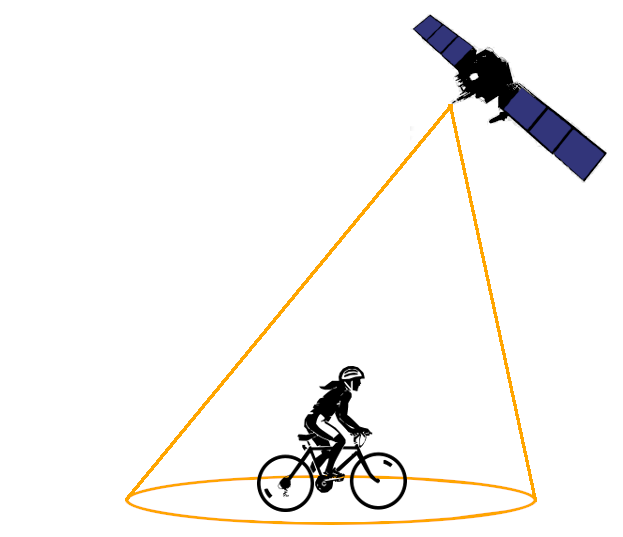
\includegraphics[width=6cm]{cyclist_just_gps.png}
\end{center}
\end{frame}

\begin{frame}{Measurement}
  \crish$$
\mathbf{X}_s\sim\mathcal{N}(\mathbf{x}_a,\mathbf{R})
$$\cbla{} {where \crish$\mathbf{R}$\cbla{} is the covariance in the
  noise in our sensor. More complex models of the sensor noise are
  often considered, but these are a straightforward extension of what
  we do here.}
\end{frame}

\begin{frame}{Bayesian fusion}
  We want to put these together.
  \crish$$p(\mathbf{x}_a|\mathbf{x}_d,\mathbf{x}_s)$$\cbla{}
From the Bayes rule:
\crish$$
p(\mathbf{x}_a|\mathbf{x}_d,\mathbf{x}_s)\propto p(\mathbf{x}_d,\mathbf{x}_s|\mathbf{x}_a)=p(\mathbf{x}_d|\mathbf{x}_a)p(\mathbf{x}_s|\mathbf{x}_a)
$$\cbla{}
\end{frame}

\begin{frame}{One-dimensional example}
  \crish$y$\cbla{}s where the \crish$\mathbf{x}$\cbla{}s are, little letters for variances, the equivalent of the covariances before.
\crish$$
p(y_a|y_d,y_s)\propto p(y_d|y_a)p(y_s|y_a)
$$\cbla{} where \crish$p(y_d|y_a)\sim\mathcal{N}(y_a,p_d)$\cbla{} and
\crish$p(y_s|y_a)\sim\mathcal{N}(y_a,r)$\cbla{}.
\vskip 1cm
This is just Bayesian fusion
\crish$$
\frac{1}{p_n}=\frac{1}{p_d}+\frac{1}{r}
$$\cbla{}
and this gives the new mean
\crish$$
\bar{y}_n=\frac{p_n}{p_d}y_d+\frac{p_n}{r}y_s
$$\cbla{}

\end{frame}


\begin{frame}{One-dimensional example}
\crish$$
\frac{1}{p_n}=\frac{1}{p_d}+\frac{1}{r}
$$\cbla{}
with new mean
\crish$$
\bar{y}_n=\frac{p_n}{p_d}y_d+\frac{p_n}{r}y_s
$$\cbla{}
We can rewrite this:
\crish$$
\frac{p_n}{p_d}=1-\frac{p_n}{r}
$$\cbla{}
so
\crish$$
\bar{y}_n=y_d+k(y_s-y_d)
$$\cbla{}
where
\crish$$
k=\frac{p_n}{r}
$$\cbla{}
Thus, the new estimate is the dead reckoning estimate along with a correction coming from the sensor. 
\end{frame}

\begin{frame}{Kalman gain}
\cblu$$
\bar{y}_n=y_d+k(y_s-y_d)
$$\cbla{}
where
\crish $$
\cblu{}k\crish=\frac{p_n}{r}\cblu=\frac{p_d}{p_d+r}
$$ \cbla{}
and
\crish$$
\frac{1}{p_n}=\frac{1}{p_d}+\frac{1}{r}
$$\cbla{}
and after a bit of algebra
\crish$$
\cblu{}p_n\crish=\frac{rp_d}{p_d+r}=\frac{p_d(r+p_d)}{p_d+r}-\frac{p_d^2}{p_d+r}\cblu=(1-k)p_d
$$\cbla{}
\end{frame}

\begin{frame}{Back to two-dimensions}
\crish$$
S=P_d+R
$$\cbla{}
and
\crish$$
K=P_dS^{-1}
$$\cbla{}
{This factor, called the \textbf{Kalman gain} is clearly the analogue of \crish$k$\cbla{} above.}
\crish$$
\mathbf{\bar{x}}_n=\mathbf{x}_d+K(\mathbf{x}_s-\mathbf{x}_d)
$$\cbla{}
and 
\crish$$
P_n=(\mathbf{1}-K)P_d
$$\cbla{}
\end{frame}

\begin{frame}{Kalman filter}
  \begin{center}
    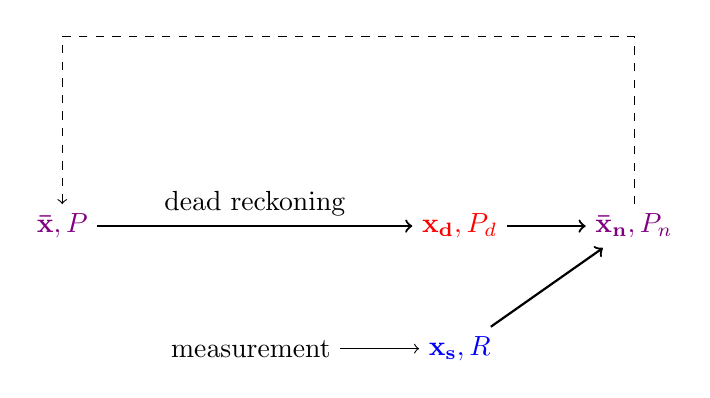
\begin{tikzpicture}
      \node[](before){\color{purple}$\mathbf{\bar{x}},P$\cbla};
      \node[right = 4cm of before](dead){\color{red}$\mathbf{x_d},P_d$\cbla};
      \node[below = 1cm of dead](sensor){\color{blue}$\mathbf{x_s},R$\cbla};
      \node[right = 1cm of dead](new){\color{purple}$\mathbf{\bar{x}_n},P_n$\cbla};
      \node[left  = 1cm of sensor](measure){measurement};
      \node[above = 2cm of new](anew){};
      \node[above = 2cm of before](abefore){};
      \draw[thick,->] (before)->node[above]{dead reckoning} (dead);
      \draw[thick,->] (dead)->(new);
      \draw[thick,->] (sensor)->(new);
      \draw[dashed,->] (new) -- (anew.center) -- (abefore.center) -> (before);
      \draw[thin,->] (measure) -> (sensor);
    \end{tikzpicture}
  \end{center}
\end{frame}



\begin{frame}{The Kalman filter and the brain}
  \begin{center}
    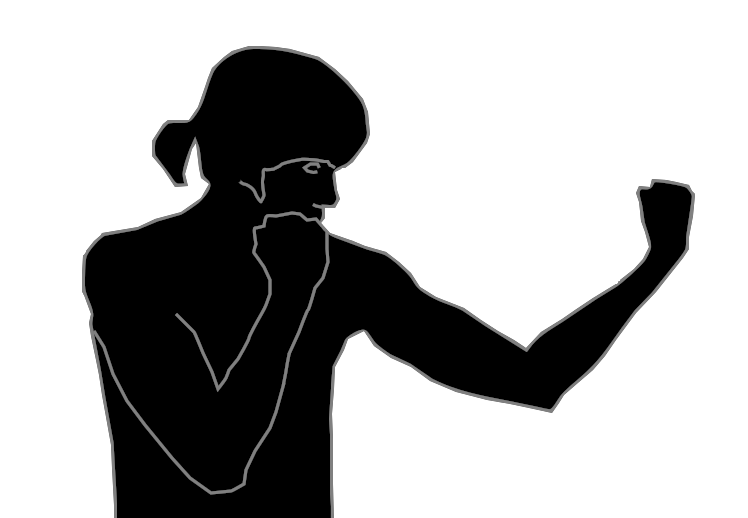
\includegraphics[width=7cm]{boxing1.png}
  \end{center}
\end{frame}


\begin{frame}{The Kalman filter and the brain}
  \begin{center}
    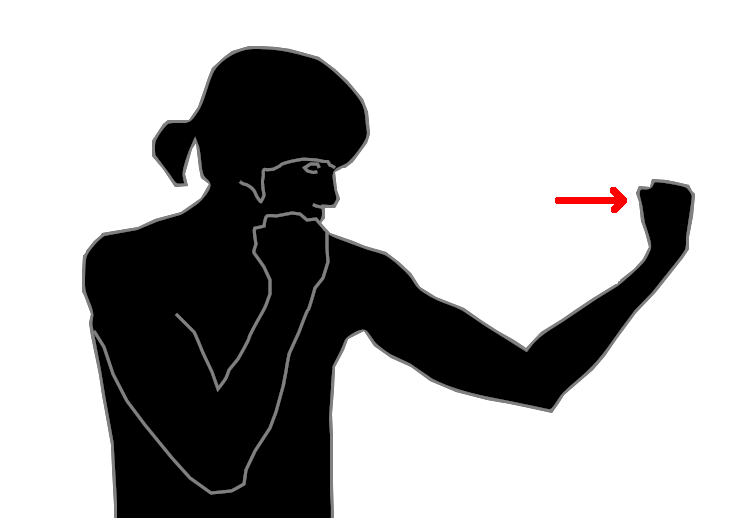
\includegraphics[width=7cm]{boxing2.png}
  \end{center}
\end{frame}


\begin{frame}{The Kalman filter and the brain}
  \begin{center}
    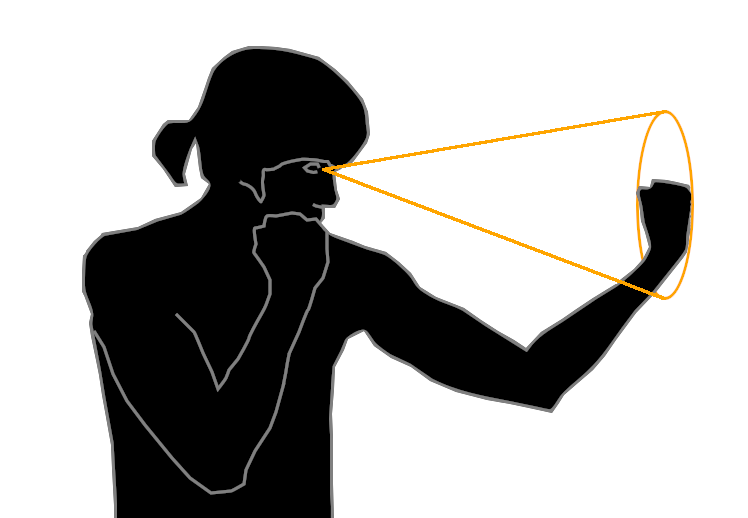
\includegraphics[width=7cm]{boxing3.png}
  \end{center}
\end{frame}


\begin{frame}{The Kalman filter and the brain}
  \begin{center}
    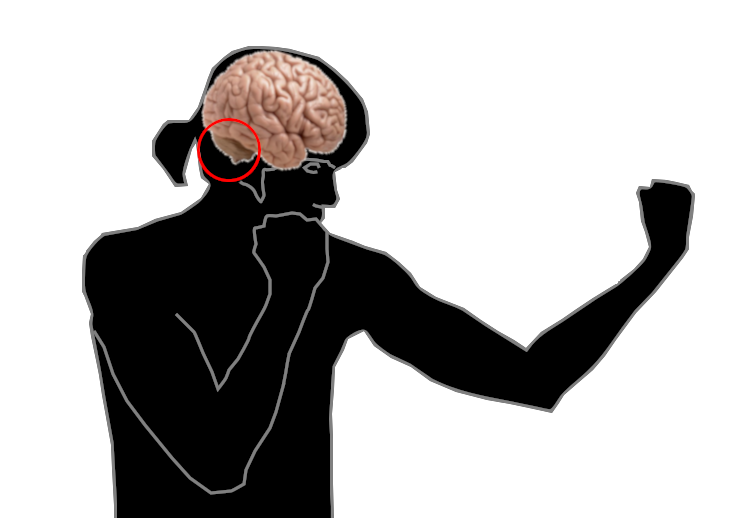
\includegraphics[width=7cm]{boxing4.png}
  \end{center}
\end{frame}

\end{document}
